\documentclass[10pt]{article}
\usepackage[utf8]{inputenc}
\usepackage[doublespacing]{setspace}
\usepackage{textcomp}
\usepackage{amsmath,amssymb,amsthm}
\usepackage{fancyhdr}
\usepackage{lastpage}
\usepackage[]{hyperref}
\usepackage[pdftex]{graphicx}
\usepackage{ctex}
\usepackage{booktabs}
\usepackage{subfigure}
\usepackage{titlesec}
\usepackage{listings}
\usepackage{enumerate}
\usepackage{bm}
\usepackage{float}
\usepackage{verbatim}
\usepackage{multirow}
%\allowdisplaybreaks
\renewcommand{\contentsname}{\centerline{Contents}}
\pagestyle{fancy}
\author{D}
\def\name{D}
\lhead{Data Mining}
\chead{}
\rhead{\name}
\cfoot{-\space\thepage\space-}
\newtheorem{exer}{\bm{$Exercise$}}
\newtheorem{prob}{\bm{$Problem$}}
\newtheorem{bonus}{\bm{$Bonus\;Problem$}}
\newcommand{\tabincell}[2]{\begin{tabular}{@{}#1@{}}#2\end{tabular}}
\CTEXoptions[today=old]

\begin{document}

\title{Assignment Two}
\date{\today}
\maketitle
\thispagestyle{fancy}
\thispagestyle{fancy}

\begin{prob}
\end{prob}
\begin{enumerate}[1)]
\vspace{3mm}

\item
R codes:
\lstinputlisting{p11a.R}
\vspace{3mm}
R outputs:
\lstinputlisting{p11b.txt}
\vspace{3mm}
Comments\footnote{ UCLA Statistical Consulting Group. (n.d.). \textit{Logit regression}. Retrieved from https://stats.idre.ucla.edu/r/dae/logit-regression/.}\footnote{ Gupta, A. (2017). \textit{Deviance and AIC for logistic regression in R}. Retrieved from https://analyticsdataexploration.com/deviance-and-aic-for-logistic-regression-in-r/.}:
\subitem
a) Calls: the model we used is a binary multiple logistic regression model.
\subitem
b) Deviation residuals: the measure of model fit, which shows the distribution of the deviance residuals for individual cases used in the model.
\subitem
c) Coefficients, standard errors, z-statistics and p-values: the coefficients of $x_1$ and $x_2$ and the intercept are statistically significant. The logistic regression coefficients give the change in the log odds of the outcome for a one unit increase in the predictor variable: for every one unit increase in $x_1$, the log odds of a forged banknote (versus a genuine banknote) decreases by 1.15591; for every one unit increase in $x_2$, the log odds of a forged banknote decreases by 0.27014.
\subitem
d) Null and deviance residuals and the AIC: null residuals measure the performance when the model includes only intercept terms and deviance residuals measure the performance when the model includes $x_1$ and $x_2$ variables; the latter is better, for $498.98<1322.01$. A model with an lower AIC is preferred when multiple models are compared.
\subitem
e) Generally, the regression has statistically significant effects.
\vspace{3mm}

\item
\subitem
i)\\
R codes\footnote{ suncoolsu. (2011). \textit{How to plot decision boundary in R for logistic regression model}. Retrieved from https://stats.stackexchange.com/q/6207.}:
\lstinputlisting{p12a.R}
\vspace{3mm}
R plots:
\begin{figure}[H]
  \centering
  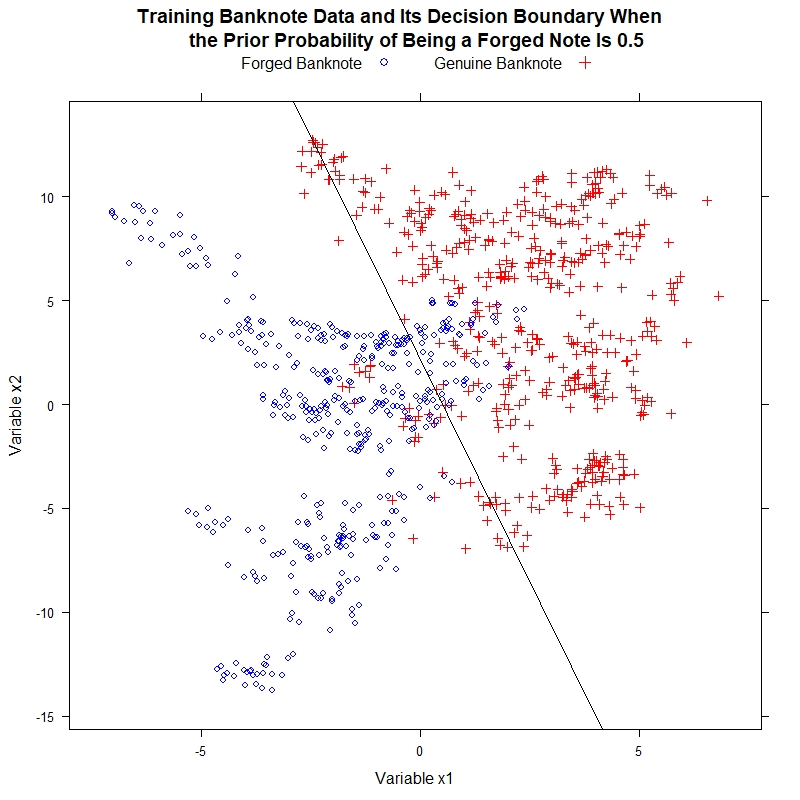
\includegraphics[width=9cm,height=9cm]{p12a.jpeg}
  \caption{Training Banknote Data and Its Decision Boundary When $\theta=0.5$}
\end{figure}

\subitem
ii)\\
R codes:
\lstinputlisting{p12b.R}
\vspace{3mm}
R outputs:
\lstinputlisting{p12c.txt}
\vspace{3mm}
The confusion matrix:\\
\begin{tabular}{llllll}
                                          &         & \multicolumn{2}{l}{True Banknote Type} &       &  \\
                                          &         & Genuine           & Forged             & Total &  \\
\multirow{2}{*}{Predicted Banknote Types} & Genuine & 216               & 27                 & 243   &  \\
                                          & Forged  & 20                & 149                & 169   &  \\
                                          & Total   & 236               & 176                & 412   &
\end{tabular}
\vspace{3mm}

Comments:
\subitem
a) The testing error rate is 0.1141 ($=(20+27)/412$) or 11.41\%. (The training error rate is 0.1177 ($=(53+60)/960$) or 11.77\%.)
\subitem
b) The accuracy is 0.8859; the misclassification rate is 0.1141.
\subitem
c) The true positive rate is 0.8466 ($=149/176$); the false positive rate is 0.0847 ($=20/236$).
\subitem
d) The true negative rate is 0.9153 ($=216/236$); the false negative rate is 0.1534 ($=27/176$).
\subitem
e) The precision is 0.8817 ($=149/169$), being acceptable; the specificity is 0.9153 ($=1-20/236$), being acceptable; the sensitivity is 0.8466, being acceptable.
\subitem
f) Generally, the logistic regression is helpful to predict if a banknote is forged or not.
\vspace{3mm}

\subitem
iii)\\
R codes:
\lstinputlisting{p12d.R}
\vspace{3mm}
R outputs:
\lstinputlisting{p12e.txt}
\vspace{3mm}
The confusion matrix using $\theta=0.6$:\\
\begin{tabular}{llllll}
                                          &         & \multicolumn{2}{l}{True Banknote Type} &       &  \\
                                          &         & Genuine           & Forged             & Total &  \\
\multirow{2}{*}{Predicted Banknote Types} & Genuine & 207               & 21                 & 228   &  \\
                                          & Forged  & 29                & 155                & 184   &  \\
                                          & Total   & 236               & 176                & 412   &
\end{tabular}
\vspace{3mm}

The confusion matrix using $\theta=0.4$:\\
\begin{tabular}{llllll}
                                          &         & \multicolumn{2}{l}{True Banknote Type} &       &  \\
                                          &         & Genuine           & Forged             & Total &  \\
\multirow{2}{*}{Predicted Banknote Types} & Genuine & 220               & 35                 & 255   &  \\
                                          & Forged  & 16                & 141                & 157   &  \\
                                          & Total   & 236               & 176                & 412   &
\end{tabular}
\vspace{3mm} % Comment: Comments?

Situations:\\
``For example, if we want to increase the number of true positives... for the default data, we could use $Pr(default=Yes|X=x)>0.2$.''\footnote{ Robertson, B. L. (2019). \textit{Lecture notes in data mining}. Unpublished manuscript.}\\
Hence, one situation that the $\theta=0.4$ model may be preferred is that in the real world the method to judge a banknote as ``genuine'' is too strict, making some genuine banknotes mislabeled as ``forged'', so in the statistical learning we want to lower the standard, increase the number of genuine banknotes and balance the result. Another situation is that the statistical analyst is bribed or threatened by the forged banknote maker who wants their illegal actions to be detected as less as possible. % Comment: wrong way round
\end{enumerate}
\vspace{3mm}

\begin{prob}
\end{prob}
\begin{enumerate}[1)]
\vspace{3mm}

\item
R codes:
\lstinputlisting{p21a.R}
\vspace{3mm}
R outputs:
\lstinputlisting{p21b.txt}
\vspace{3mm}
The probability of a banknote being forged is 0.4029 ($=166/412$)\\
The confusion matrix:\\
\begin{tabular}{llllll}
                                          &         & \multicolumn{2}{l}{True Banknote Type} &       &  \\
                                          &         & Genuine           & Forged             & Total &  \\
\multirow{2}{*}{Predicted Banknote Types} & Genuine & 216               & 30                 & 246   &  \\
                                          & Forged  & 20                & 146                & 166   &  \\
                                          & Total   & 236               & 176                & 412   &
\end{tabular}
\vspace{3mm}

\item
R codes:
\lstinputlisting{p22a.R}
\vspace{3mm}
R outputs:
\lstinputlisting{p22b.txt}
\vspace{3mm}
The probability of a banknote being forged is 0.4005 ($=165/412$)\\
The confusion matrix:\\
\begin{tabular}{llllll}
                                          &         & \multicolumn{2}{l}{True Banknote Type} &       &  \\
                                          &         & Genuine           & Forged             & Total &  \\
\multirow{2}{*}{Predicted Banknote Types} & Genuine & 219               & 28                 & 247   &  \\
                                          & Forged  & 17                & 148                & 165   &  \\
                                          & Total   & 236               & 176                & 412   &
\end{tabular}
\vspace{3mm}

\item
Comments:
\subitem
a) The testing error rate is 0.1214 for LDA and 0.1092 for QDA.
\subitem
b) The accuracy is 0.8786 and 0.8908 respectively; the misclassification rate is 0.1214 and 0.1092 respectively.
\subitem
c) The true positive rate is 0.8295 and 0.8409 respectively; the false positive rate is 0.0847 and 0.0720 respectively.
\subitem
d) The true negative rate is 0.9153 and 0.9280 respectively; the false negative rate is 0.1705 and 0.1591 respectively.
\subitem
e) The precision is 0.8795 and 0.8970 respectively; the specificity is 0.9153 and 0.9280 respectively; the sensitivity is 0.8295 and 0.8409 respectively.
\vspace{3mm}

Recommendation:\\
To sum up, I create a table.\\
%The accuracy of the logistic regression method is 0.8859; the accuracy of the LDA method is 0.8786 ($=362/412$); the accuracy of the QDA method is 0.8908 ($=369/412$); the other parameters can found above.
\begin{tabular}{llllll}
                    & Accurracy       & Error Rate      & Precision       & Specificity     & Sensitivity     \\
LR                  & 0.8859          & 0.1141          & 0.8817          & 0.9153          & \textbf{0.8466} \\
LDA                 & 0.8786          & 0.1214          & 0.8795          & 0.9153          & 0.8295          \\
QDA                 & \textbf{0.8908} & \textbf{0.1092} & \textbf{0.8970} & \textbf{0.9280} & 0.8409
\end{tabular}
\vspace{3mm}

If comparing the accuracy (or the testing error rate equivalently), the precision and the specificity, I vote for the QDA method; if comparing the sensitivity, I vote for the logistic regression. In all, I recommend the QDA method for this problem. % Comment: OK

\end{enumerate}
\vspace{3mm}

\begin{prob}
\end{prob}
\begin{enumerate}[1)]
\vspace{3mm}

\item
R codes:
\lstinputlisting{p31a.R}
\vspace{3mm}
R outputs:
\lstinputlisting{p31b.txt}
\vspace{3mm}
The confusion matrix:\\
\begin{tabular}{llllll}
                                          &         & \multicolumn{2}{l}{True Classes}        &       &  \\
                                          &         & Class 0           & Class 1            & Total &  \\
\multirow{2}{*}{Predicted Classes}        & Class 0 & 660               & 60                 & 720   &  \\
                                          & Class 1 & 125               & 1156               & 1281  &  \\
                                          & Total   & 775               & 1216               & 2001  &
\end{tabular}
\vspace{3mm}

The testing error rate for QDA is 0.0925 ($=(60+125)/2001$).
\vspace{3mm}

\item
R codes:
\lstinputlisting{p32a.R}
\vspace{3mm}
R outputs:
\lstinputlisting{p32b.txt}
\vspace{3mm}
The confusion matrix:\\
\begin{tabular}{llllll}
                                          &         & \multicolumn{2}{l}{True Classes}       &       &  \\
                                          &         & Class 0           & Class 1            & Total &  \\
\multirow{2}{*}{Predicted Classes}        & Class 0 & 500               & 250                & 750   &  \\
                                          & Class 1 & 285               & 966                & 1251  &  \\
                                          & Total   & 785               & 1216               & 2001  &
\end{tabular}
\vspace{3mm}

The testing error rate for LDA is 0.2674 ($=(250+285)/2001$).
\vspace{3mm}

Comments:
\subitem
a) The QDA model generates a better result, for its less errors (less false negatives and more true positives).
\subitem
b) The reasons that QDA generates a better result are possibly that the large amount of data (2001) fits QDA better than LDA and data with varying covariance (generating more than one decision boundary) fits QDA better than LDA. % Comment: This is not the correct approach - see the model answers.

\end{enumerate}

\end{document}
